%\Documentclass[12pt]{jreport}
\documentclass[uplatex, 12pt]{ujbook}
%%
%%  卒業論文 スタイルファイル 2020年度版
%%                       T. MATSUZAKI
%%  $Lastupdate: Fri Nov  6 11:37:15 2020 $
%%
%\begin{figure}[htpb]
% \begin{center}
%  \includegraphics[width=8cm,height=4cm,clip,keepaspectratio]{syouroku.eps}
% \end{center}
% \caption{図3.1}
% \label{fig:FIG1}
%\end{figure}

\usepackage{jgraduate20}     % jgraduate20.styを読み込む
\usepackage[dvipdfmx]{graphicx}
\usepackage{makeidx}          % 索引作成用
%\usepackage{url}             %いらないかも
\usepackage[hang,small,bf]{caption}
\usepackage[subrefformat=parens]{subcaption}
\captionsetup{compatibility=false, labelsep=space} %←先生のスタイルファイルと競合回避のために書き換え（:が表示されないように）

% 前設定
\usepackage[
    dvipdfmx,			% PDFを作る方法（ドライバ）を指定
    bookmarks=true,		% PDFにしおり（目次）を自動作成
    bookmarksnumbered=true,	% しおりに章番号 (1.1など) を付ける
    colorlinks=true,		% リンクを色付きテキストにする (枠線を消す)
    linkcolor=black,		% 目次や本文中 (\ref) のリンクを黒色に
    citecolor=black,		% 参考文献 (\cite) へのリンクを黒色に
    urlcolor=black		% URL (https://...) のリンクを黒色に
]{hyperref}
\usepackage{pxjahyper}	%文字化け防止

\doubleside{1}                % 1:両面印刷/0:片面印刷

\title{13.56MHz高周波電源の出力最大化に向けた自動整合器の製作}
\authorid{2211170029}
\author{永野　優翔}
\university{近畿大学}                 % 大学名 (近畿大学, etc.)
\department{産業理工学部}             % 学部名 (産業理工学部, etc.)
\major{電気電子工学科}                % 学科名 (電気電子工学科, etc.)
%\date{\today}
\date{令和7年 1月15日}
\year{令和七年度}
\teacherpos{教授}
\teacher{喜屋武　毅}
\coauthornum{2}                       % 共同研究者の人数 (2人まで対応)
\cfauthid{2211170053}                % 共同研究者1の学籍番号
\cfauth{貴船 芳尚}                    % 共同研究者1の名前
\csauthid{2211170054}                % 共同研究者2の学籍番号
\csauth{中尾 楓}                    % 共同研究者2の名前          

\begin{document}
\maketitle                    % 表紙
\cleardoublepageskip          % 両面印刷の場合表紙の裏は白紙にします
\tableofcontents              % 目次 (↓ *のついている項目)
\listoffigures                % 図目次
\listoftables                 % 表目次
\cleardoublepageskip          % 目次と本文を分離・両面印刷の場合表紙の裏は白紙にします
\pagenumbering{arabic}        % ページ番号をアラビア数字に
\newpage

%===============================================================
\chapter{序章}

\section{本研究の背景}
 近年,AIやlot技術の急速な発展に伴い,その基盤となる半導体デバイスの需要は飛躍的に
 増加している.半導体の高性能化と高集積化を達成するため,微細化する技術がふかけつであり,
 その中核を担うのが高周波プラズマプロセスである.このプラズマ生成プロセスにおいて,
 RF電源から負荷へと電力を効率よく伝送するためには,インピーダンス整合が極めて重要となる.
 RF電源の伝送線路は通常50Ωで設計されるが,負荷であるプラズマのインピーダンスは,点火の瞬間,
ガスの種類,圧力,投入電力などの実験条件のわずかな変化により常に変動する.プラズマ側で
インピーダンスが整合しない場合,供給電力の一部が反射電力として電力側に戻ってしまう.
この反射電力は伝送効率の著しい低下を招くだけではなく,RF電源や関連部品の発熱・故障を引き起こす.
そのため,安定した半導体製造プロセスを実現するためには,負荷の変動に追従し,反射電力を抑制する
インピーダンス自動整合器が必要不可欠となっている.\\従来の整合技術には,調整に時間を要し変動に
追従できない手動整合器,効果で制御がブラックボックス化された市販の自動整合器という課題が存在する.
さらに,本研究室において,RF電源と負荷の特性を評価するための50Ωに整合された標準的な測定・制御環境
が整備されていない.\\ 
本研究では,これらの課題を解決し,研究室における50Ωの標準的なRF整合環境を
確立することを第一の目標とし,自動整合器の製作を行う.

\section{本研究の目的}
 13.56MHz高周波電源の出力最大化

\section{本論文の構成}
 本論文では、第１章｢序論｣,第２章｢自動整合器の概要｣,第３章「自動整合器の設計｣,
 第４章｢自動整合器の動作と評価｣,第５章｢結論｣の５章から構成されている.
 第２章では,自動整合器の４つの部門の役割について述べる.第３章では各部門の設計に述べ,
 第４章で各部門の計測をおこない,その結果の評価について述べる.第５章で各章の総括を述べる.
%====================================================================
\chapter{自動整合器の概要}

\section{自動整合器の構成}
 自動整合器は大きく４つの部門で構成されている.図2.1に自動整合器の構成図を示す.
 自動整合器ではRF電源から電力が送られ,反射波検出部を通って負荷側へと行く.整合が取れていない場合,
 負荷側からの反射波を反射波検出部によって検出する.検出された反射波の信号を処理・制御部で受信,
 処理を行う.その後処理された信号は駆動部に送られ,処理・制御部で処理された信号によって駆動部の
 モータを動かし整合回路部の可変コンデンサとコイルを用いて自動でインピーダンス整合を行う.
 \begin{figure}[!b]
 \begin{center}
  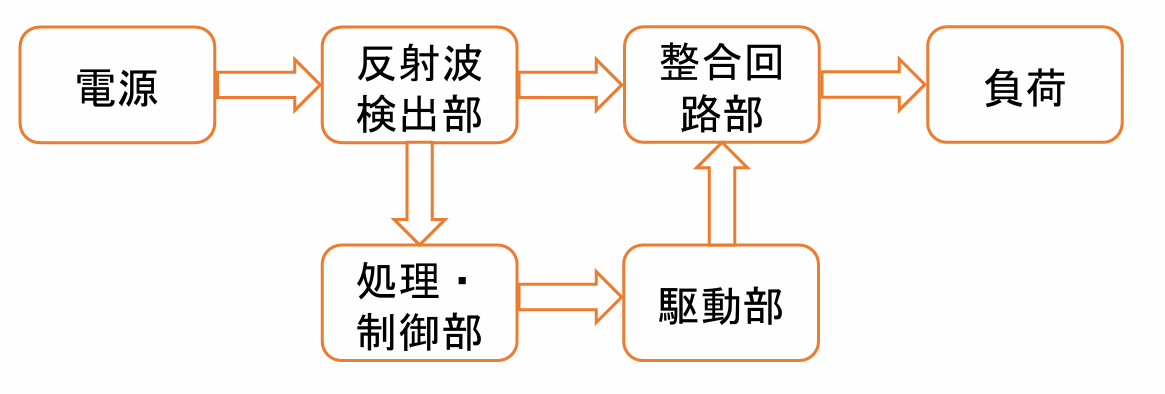
\includegraphics[width=18cm,height=10cm,clip,keepaspectratio]{2.1.png}
 \end{center}
 \caption{自動整合器の構成図}
 \label{fig:2.1}
\end{figure}
%-------------------------------------------------------------------------
\section{反射波検出部}
 \subsection{方向性結合器の原理}
 方向性結合器は,伝送線路を流れる高周波信号を,進行波成分と反射波成分に相互に影響を与えることなく
 分離し,それぞれの電力値を正確に検出するために不可欠なものである.本研究で開発する自動整合器において
 負荷の整合状態を把握するために必要である.\\
 
 \subsection{方向性結合器の動作}
 方向性結合器は,4ポートによって構成される.\\\\
 1. ポート１（入力）：RF電源からの電力供給点.\\
 2. ポート２（出力）：負荷への接続点.\\
 3. ポート３（進行波検出）：順方向（ポート１から２）の信号を検出.\\
 4. ポート４（反射波検出）：逆方向（ポート２から１）の信号を検出.\\\\
 方向性結合器は,CM型やタンデム型などの種類があるが,本研究では設計の容易性などを考慮してタンデム型を
 採用した.タンデム型方向性結合器は伝送線路を流れる高周波信号を,進行波と反射波あの成分に分離し,
それぞれの電力値を正確に整合状態を把握するためのフィードバック信号を提供するものである.\\

進行波と反射波の分離理論は二つの検出信号$V_v$と$V_i$を用いて,以下の理論に基づき信号を分離する.ここで,
$K_v$と$K_i$はそれぞれの検出部の結合係数である.\\\\
1. 進行波の検出（$V_f$）:進行は検出ポートの信号$V_f$は,電圧信号$V_v$と電流信号$V_i$を同相で合成することで
得られる.\\
\begin{equation}
    V_{f} = K_{v}V + Z_{0}K_{i}I
    \label{ed:2.2.1}
\end{equation}
この合成により,進行波成分は合成され,反射波成分は位相が反転しているため打ち消される.\\\\
2. 反射波の検出（$V_r$）:反射波検出ポートの信号$V_r$は,電圧信号$V_v$と電流信号$V_i$を逆相で合成することで
得られる.\\
\begin{equation}
    V_{r} = K_{v}V - Z_{0}K_{i}I
    \label{eq:2.2.2}
\end{equation}
この合成により,反射波成分は合成され,進行波成分は打ち消される.\\
理想的な分離を実現するためには,結合係数が$K_v$=$K_i$となるように,回路パラメータを精密に調整する必要がある.
本研究ではトロイダルコアを用いて実現し,13.56MHz帯の高電力かつ安定した動作を目指した.
伝送線路内の進行電力$P_f$と反射電力$P_r$とすると,方向性結合器の性能は以下の2つの主要な指標によって定義される.\\\\
1. 結合度（C）：主線路の電力に対する検出ポートの電力の比率を示す.本研究では,測定の容易性と回路の実現性を
考慮し,適切な結合度を設計した.
\begin{equation}
  C = 10 \log_{10} \left( \frac{P_r}{P_f} \right) \quad [\mathrm{dB}]
  \label{eq:2.2.3}
\end{equation}\\
2. 方向性（D）：結合器の分離性能を示す最も重要な指標である.理想的には無限大が望ましいが,実現には有限の
値となる.この値が高いほど,不要な漏れが少なく,検出精度が高いことを意味する.
 \begin{figure}[!h]
 \begin{center}
  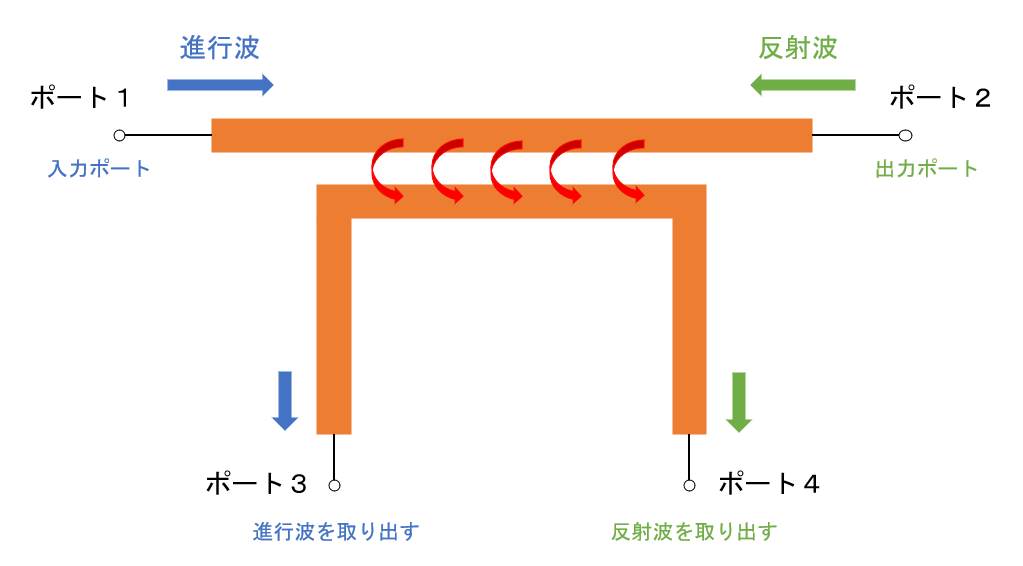
\includegraphics[width=14cm,height=8cm,clip,keepaspectratio]{2.2.png}
 \end{center}
 \caption{方向性結合器の構成図}
 \label{fig:2.2}
\end{figure}
%-------------------------------------------------------------------------------
\section{整合回路部}
 \subsection{整合回路部の概要}
整合回路は,高周波電力伝送システムにおいて,電源側と負荷との間にあり,インピーダンスの不一致を解消し,
最大電力伝送を実現するために不可欠な回路である.

基本的にリアクタンス素子であるインダクタンス（L）と
キャパシタンス（C）のみを用いて構成される.リアクタンス素子は,電力を消費しないため,整合回路自体で
エネルギーを無駄に消費することなく,インピーダンスの実数部と虚数部を変換できる.整合回路の代表的な
構造として,L型,T型,π型マッチング回路がある.
 \subsection{整合回路部の種類}
 1. L型整合回路\\

2つのリアクタンス素子をL字型に組み合した最も基本的な整合回路であり,1つの直列素子と1つの並列素子で
構成される.構造が最も単純で,調節が比較的容易であるが,整合できるインピーダンスの範囲が限られているため,
負荷インピーダンスが大きく変動する環境では不向きという欠点がある.\\

2.T型整合回路\\

2つの直列素子の間に1つの並列素子を挟んだ構造で自由度があり,広範囲のインピーダンス整合が可能である.
特に,目標インピーダンスよりも低いインピーダンスに変換する際に適している.整合範囲が広いことに伴い,
変換比が大きいとロスが生じるという欠点がある.\\

3.π型整合回路\\

3つの素子のうち,2つの素子を独立して調整できる自由度を持つ.L型整合回路よりも広範囲な負荷インピーダンス変動
に対応可能であるため,プラズマ負荷のように変動が大きい環境で採用される.T型整合回路同様に,整合範囲が広い
ため変換率が大きいとロスが生じるという欠点がある.\\

本研究では,π型整合回路が一般的な自動整合器に使われている点,整合範囲が広範囲である点からπ型整合回路を
採用した.\\
\begin{figure}[!h]
 \begin{center}
  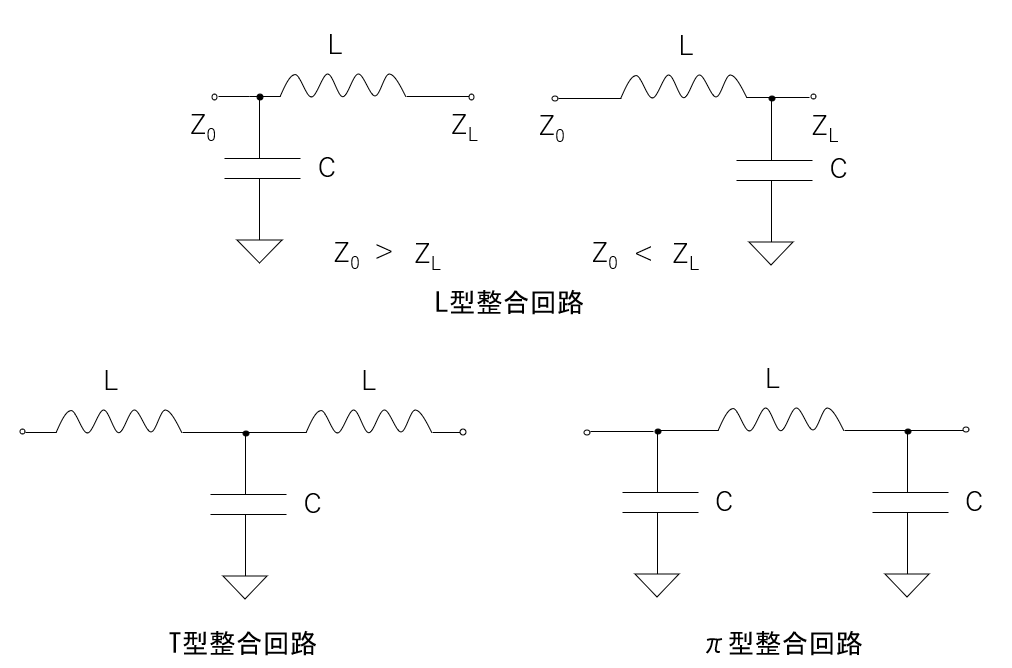
\includegraphics[width=13cm,height=10cm,clip,keepaspectratio]{2.3.png}
 \end{center}
 \caption{L型,T型,π型整合回路図}
 \label{fig:2.3}
\end{figure}
%-------------------------------------------------------------------------------
\section{駆動部}
 \subsection{駆動部の概要}
 駆動部は,処理・制御部の制御アルゴリズムによって計算された最適な容量値に,モーターを用いて整合回路部の可変コンデンサを
調整する役割を担う.\\
 \subsection{駆動部の動作}
 駆動部に要求される性能として以下の通りである.\\\\
1.バリコンを精密に動かす高精度な位置決めが必要である.\\
2.整合が完了した後に停止位置の保持が必要である.\\
3.制御をするうえで,複雑すぎない制御アルゴリズムである必要がある.\\

以上の3点を踏まえて,本研究ではステッピングモーターを採用した.\\
ステッピングモーターは磁極が段階的に移動して一定角度で回転し,高精度な位置決めと停止時の位置保持が可能である.

また,制御を容易にするためモーター駆動をするにあたって,今回はモータードライバーを介して制御を行った.
%--------------------------------------------------------------------------------
\section{処理・制御部}
 \subsection{処理・制御部の概要}
処理・制御部は方向性結合器から得られた反射電力を検出し,その信号をマイコンで受信,処理される.処理された信号は
モータードライバーに送られ,モーター,可変コンデンサを制御する.そのほか,整合中や整合完了を知らせるためのLED,
反射電力などを表示するLCDの制御も行う.
 \subsection{最適点の探索}
処理・制御部で方向性結合器を用いて反射波を測定し,小さくなる方向を見つけ,最適点を探す必要がある.
最適点を探す手段として以下に示す.\\

1.グリッドサーチ法

π型整合回路の２つの可変コンデンサのすべての組み合わせを試し,その中で一番反射波が少ない組み合わせを最適点とする.
しかし,すべての組み合わせを試すため,見つけるまでに時間を要する.\\

2.最適化式から最適点を探す方法

反射波,位相などの値を数式を用いて計算して最適点を探す.計算で探すため,理論的には1回で最適点を見つけることができ,
高速で,正確な整合が可能である.しかし,位相や最適化式の導出が高度である.\\

3.山登り法

π型回路の可変コンデンサを少しずつ変化させて,反射電力の変化に基づいて戻る,進むを繰り返し最適点を探す.
反射波の情報だけで制御できるため,比較的容易に構成できる.しかし,初期位置や負荷条件によっては局所解に陥り,
最適点にたどり着かない可能性がある.\\

本研究では以上の3つを比較し最適点の導出にあたって,回路の容易性,整合時間などを考慮し山登り法を採用した.
%=================================================================================
\chapter{自動整合器の設計}

\section{自動整合器の仕様}
 いかに示すのは設計した自動整合器の仕様である.\\\\
・  動作周波数         13.56[MHz]\\
・  最大入力電圧       122[V]\\ 
・  目標インピーダンス　50[Ω]\\
・  整合可能範囲       R=50～300[Ω], X=－100～150[Ω] (Z≒50～330[Ω])
%------------------------------------------------------------------------------------
\section{反射波検出部}
 \subsection{設計した方向性結合器の概要}
 本研究で設計した方向性結合器はタンデム型方向性結合器を採用した.タンデム型は電圧検出トランスと電流検出トランスの
 二つの検出器を組み合わせて,進行波と反射波の電圧・電流成分を合成・分離する.

 実際に設計した方向性結合器の結合度は一般的な指標である20dBを目標にした.タンデム型における結合度は,巻線数(N)に大きく依存し
 以下の式で表される.
 \begin{equation}
  C \approx 20 \log_{10} (N)
  \label{eq:3.1}
\end{equation}

\newpage

これをもとに目標の20dBを得るため巻線数を10回巻にした.

また一次側と二次側のインダクタンス比を1:100で設定し,値は一次側を0.557μH,
二次側を55.7μHとした.ここで周波数f=13.56MHzでリアクタンス$X_L$=2πfLをそれぞれ計算すると,

\begin{equation}
 X_L = 2\pi \times (13.56 \times 10^6) \times (0.557 \times 10^{-6}) \approx 47.4 \, \Omega
  \label{eq:3.2}
\end{equation}

\begin{equation}
 X_L = 2\pi \times (13.56 \times 10^6) \times (55.7 \times 10^{-6}) \approx 4700 \, \Omega
  \label{eq:3.3}
\end{equation}\\\\
となり,13.56MHzにおいて$X_L$=47.4Ωとなることは目標とする50Ωに近い値である.また,検出側の回路設計においては主線路の状態を
正確に反映させるため,特性インピーダンスの3倍以上の値にする必要があり$X_L$=4700Ωと十分に大きい値となる.これに伴って製作を行った.

製作するにあたり,検出トランスコアには高い透磁率を持ち,数MHzから数十MHz帯域でのRF用途に広く適応しているフェライトコアFT114-43材を
使用した.\\\\
\begin{figure}[!h]
 \begin{center}
  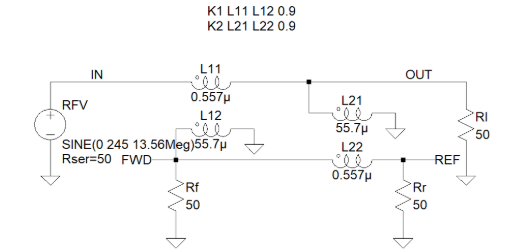
\includegraphics[width=10cm,height=10cm,clip,keepaspectratio]{3.1.png}
 \end{center}
 \caption{製作した方向性結合器}
 \label{fig:3.1}
\end{figure}
 \subsection{設計した検波回路}
 本研究では,方向性結合器からの信号を「Arduino R4」の最大定格電圧(5V)以下に下げる必要があり検波回路を製作した.今回製作した
 検波回路は「検波回路」,「LPF」,「分圧回路」から構成されている.

 検波回路は13.56MHzの高周波でも対応可能な「BAT54」のショットキーダイオードで設計を行った.実際の検波回路には「BAT54」と
 同等の特性を持つ「BAT43」を使用した.

 LPFは13.56MHzでの高周波ひずみを低減を目的とするために設けた.検波回路に影響が少なく,研究室にある値で設計を行った.

 分圧回路は5(V)以下に電圧を下げる目的とするために設けた.分圧比は,直列抵抗$R_{d1}$,接地抵抗$R_{d2}$とすると,
 
 \begin{equation}
 Ratio = \frac{R_{d2}}{R_{d1} + R_{d2}}
  \label{eq:3.4}
\end{equation}\\

となり,安全マージンを考慮してシミュレーションを行った結果,以下の値で設計した.

\begin{equation}
 R_{d1} = 22\,\mathrm{k} + 10\,\mathrm{k} + 5.6\,\mathrm{k} = 37.6\,\mathrm{k}\Omega
  \label{eq:3.5}
\end{equation}

\begin{equation}
 R_{d2} = 47\,\mathrm{k}\Omega
  \label{eq:3.6}
\end{equation}

\begin{equation}
 \mathrm{Ratio} = \frac{47}{37.6 + 47} \approx 0.556 = 56\,\%
  \label{eq:3.7}
\end{equation}\\

\begin{figure}[h!]
 \begin{center}
  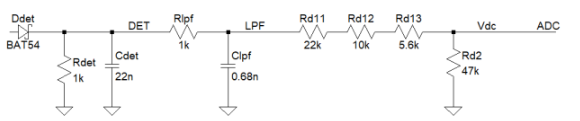
\includegraphics[width=15cm,height=10cm,clip,keepaspectratio]{3.2.png}
 \end{center}
 \caption{製作した検波回路の全体図}
 \label{fig:3.2}
\end{figure}
 %----------------------------------------------------------------------------
\section{整合回路部}
 \subsection{整合範囲}
 整合回路の設計に伴い,整合範囲を設定する必要がある.本研究では,特に半導体プロセスなどで広く用いられる
 低気圧プラズマ負荷を対象とした.低気圧プラズマ負荷は,点火時には高インピーダンス状態から急激に低インピ
 ーダンス状態へと変化するため,広範囲で整合を取る必要がある.以上の点を踏まえて,スミスチャートを
 もとに整合範囲を定め以下に示す.\\

  ・R=50～300[Ω] 

  ・X=－100～150[Ω] (Z≒50～330[Ω])\\

 \begin{figure}[h!]
 \begin{center}
  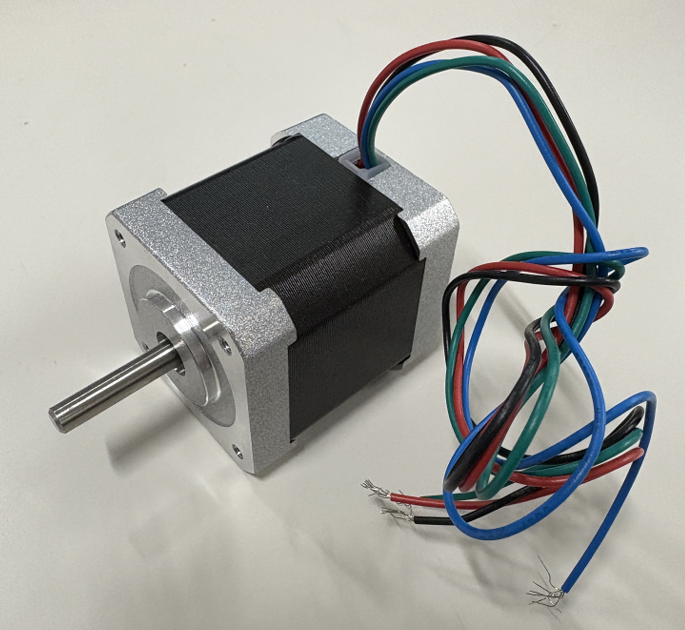
\includegraphics[width=10cm,height=10cm,clip,keepaspectratio]{3.3.png}
 \end{center}
 \caption{スミスチャートで示した整合範囲}
 \label{fig:3.3}
\end{figure}
 \subsection{コイルとコンデンサの選定}
 3.3.1で示した整合範囲を可能にするためコイルとコンデンサをπ型整合回路で製作を行った.π型整合回路では
 1つのコイルと2つの可変コンデンサからなる回路である.13.56MHzの周波数で低気圧プラズマ負荷との整合をとる
 際,インピーダンスが非常に広い範囲で変動することが予想される.そのため本研究では,コンデンサ1（）,
 コンデンサ2（）,の二つの可変コンデンサを選定した.この２つのコンデンサは整合範囲を十分に満たす.
 また,シミュレーションの結果からコイルの固定値は0.6μHとし,塩ビパイプにポリエステル銅線の巻きつけて
 製作した.製作後の実測値は0.65μHである.

 \begin{figure}[htpb]
 \centering
  
 \begin{minipage}[b]{0.45\textwidth}
  \centering
  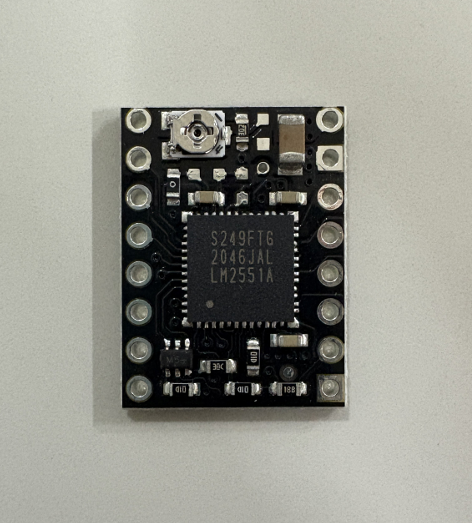
\includegraphics[width=\textwidth]{3.4.png}
  \subcaption{コンデンサ1}
  \label{fig:3.4}
 \end{minipage}
 \hfill
 \begin{minipage}[b]{0.45\textwidth}
  \centering
  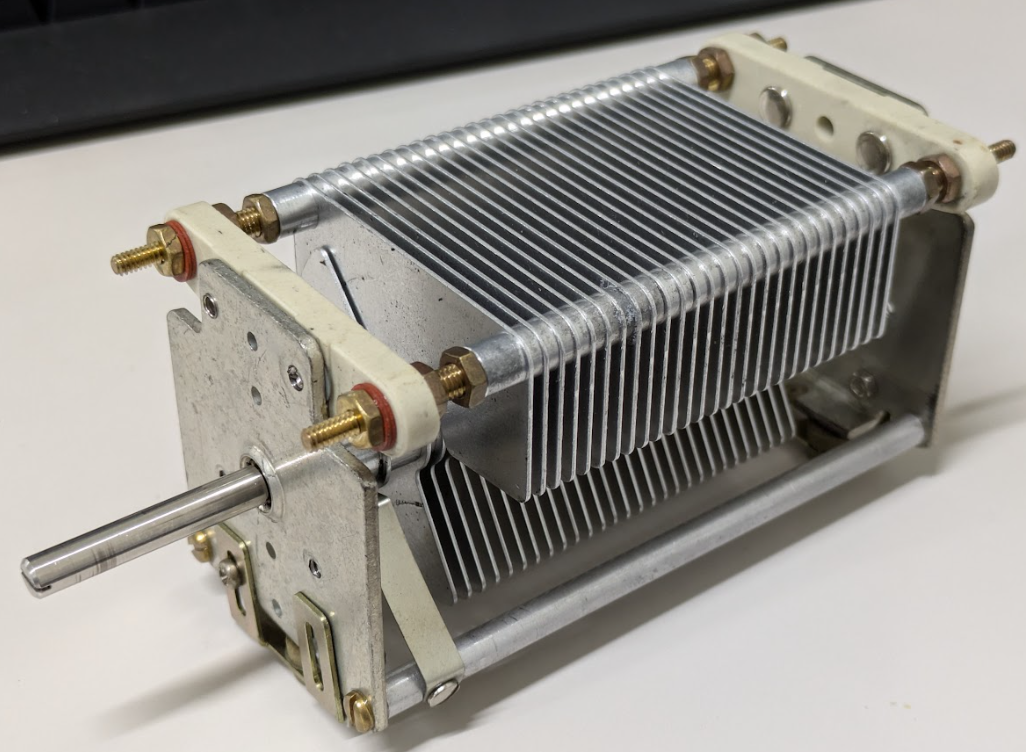
\includegraphics[width=\textwidth]{3.5.png}
  \subcaption{コンデンサ2}
  \label{fig:3.5}
 \end{minipage}
  
 \caption{可変コンデンサ}
 \label{fig:two_images}
\end{figure}

\begin{figure}[h!]
 \begin{center}
  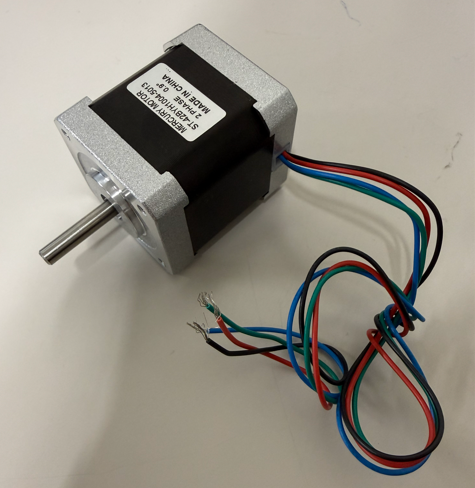
\includegraphics[width=10cm,height=8cm,clip,keepaspectratio]{3.6.png}
 \end{center}
 \caption{コイル}
 \label{fig:3.6}
\end{figure}
 %-----------------------------------------------------------------------------------
\section{駆動部}
 \subsection{ステッピングモータの選定}
 本研究ではバイポーラステッピングモータ（ST-42BYH1004）を採用した.

 モータの選定において求める条件として,可変コンデンサを動かすだけのトルクと整合完了後に値が変動しないための
 位置保持ができるものである.図3に示す選定した（ST-42BYH1004）の保持トルクは43.12[N・cm]であり
 今回使用した可変コンデンサのトルクの1.94[N・cm]を十分満たしている.また,2.4.2で示した駆動部に要求される性能も十分に
 満たしていることから,今回は（ST-41BYH1004）を採用した.\\
 \begin{figure}[h!]
 \begin{center}
  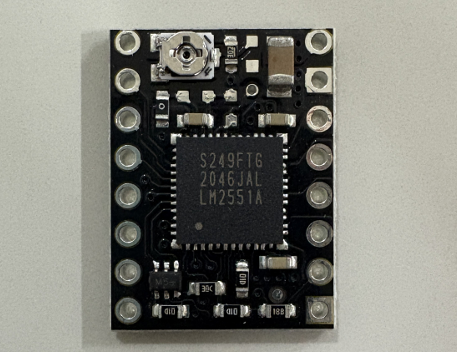
\includegraphics[width=10cm,height=6cm,clip,keepaspectratio]{3.7.png}
 \end{center}
 \caption{バイポーラステッピングモータ（ST-42BYH1004）}
 \label{fig:3.7}
\end{figure}

\subsection{モータドライバの選定}
 3.4.1で選定したバイポーラステッピングモータを駆動させる素子としてモータドライバ（TB67S249FTG）を採用した.

処理・制御部のマイコンとモータは直接駆動させることができないため,間にモータドライバを設けてモータ駆動を実現した.\\
\begin{figure}[!h]
 \begin{center}
  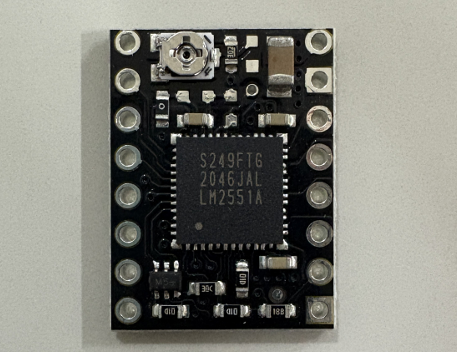
\includegraphics[width=6cm,height=6cm,clip,keepaspectratio]{3.8.png}
 \end{center}
 \caption{モータドライバ}
 \label{fig:3.8}
\end{figure}

\newpage

 \subsection{モータ周りの諸部品}
 本研究で製作する自動整合器では電源を入れた際に可変コンデンサの現在位置を把握し整合を開始する必要がある.可変コンデンサの
 位置を把握するため,初期位置を設け電源を入れると初期位置に戻るプログラムにした.その際に,初期位置を検出するセンサとして
 透過型フォトセンサを設けた.フォトセンサは発光素子と受光素子間で3Dプリンタで製作した1か所だけスリットを設けた円盤を使い,
 光の遮断,透過を認識する.スリットを設けた場所を可変コンデンサの初期位置とした.

 また,バイポーラステッピングモータと可変コンデンサを絶縁カップリングで接続し,軸の高さを合わせ,モータ駆動による
 振動がある場合でも互いの軸が同じ高さのままで固定されるようにした.\\\\\\
 \begin{figure}[!h]
 \begin{center}
  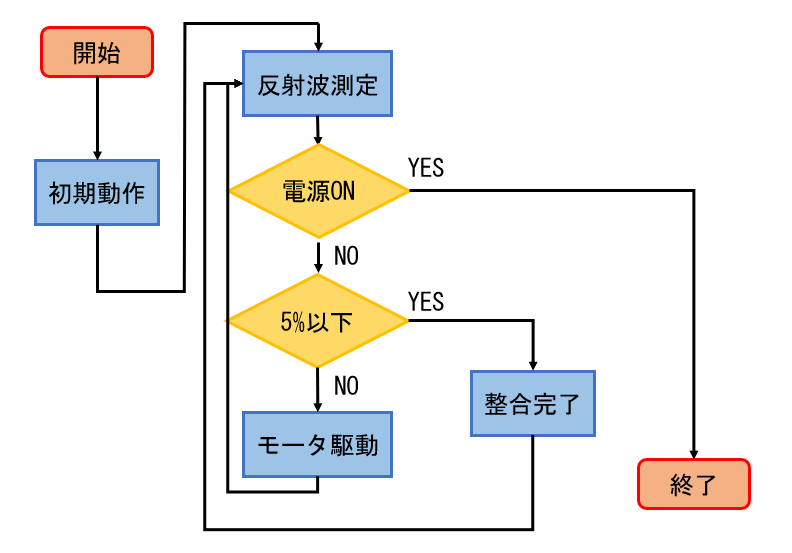
\includegraphics[width=8cm,height=6cm,clip,keepaspectratio]{3.9.png}
 \end{center}
 \caption{モータ周りの諸部品}
 \label{fig:3.9}
\end{figure}

\newpage
 %--------------------------------------------------------------------------------------------------
 \section{処理・制御部}
 \subsection{Arduinoのアルゴリズム}
処理・制御部では主に以下の4つを行う.\\
・反射波成分の取得\\
・制御アルゴリズムによる判定（山登り方）\\
・駆動部パルスの生成と送信（モータドライバに送信するパルスでモータを動かす）\\
・LCRモニタ,LEDによる状態の表示\\


これらを動作するにあたって,「Arduino R4」,「Arduino R3」,「STM32」の3つが候補として挙げられる.


反射波成分の取得に関して「許容電圧」,「ADCの分解能」,「ADC変換速度」の精度をそれぞれ以下の表にまとめる.\\


\begin{table}[!h]
    \centering
  \caption{Arduino R4,R3,STM32の特性}
  \label{tab:3.5.01}
  \begin{tabular}{|c||c|c|c|}
    \hline
    \textbf{項目} & \textbf{Arduino R4} & \textbf{Arduino R3} & \textbf{STM32} \\
    \hline\hline % 二重線
    許容電圧 & 0$\sim$5V & 0$\sim$5V & 0$\sim$3.3V \\
    \hline
    ADCの分解能 & 10, 12, 14bit & 10bit & 12bit \\
    \hline
    ADC変換速度 & 20$\sim$40us & 100us弱 & 最速1us \\
    \hline
  \end{tabular}
\end{table}

分解能に関して,「Arduino R4」,「STM32」が精度が良い.次に変換速度に関して,「STM32」が最速1μsであり一番精度が
よく,2.5.2で示した最適化式から最適点を探す方法に向いている.しかし,本研究では回路の容易性,整合時間などを考慮して
山登り方を採用したため「STM32」ほどの変換速度は必要ではない.以上の理由から本研究では「Arduino R4」を採用した.

図3.7にフローチャートを示す.

 \begin{figure}[!h]
 \begin{center}
  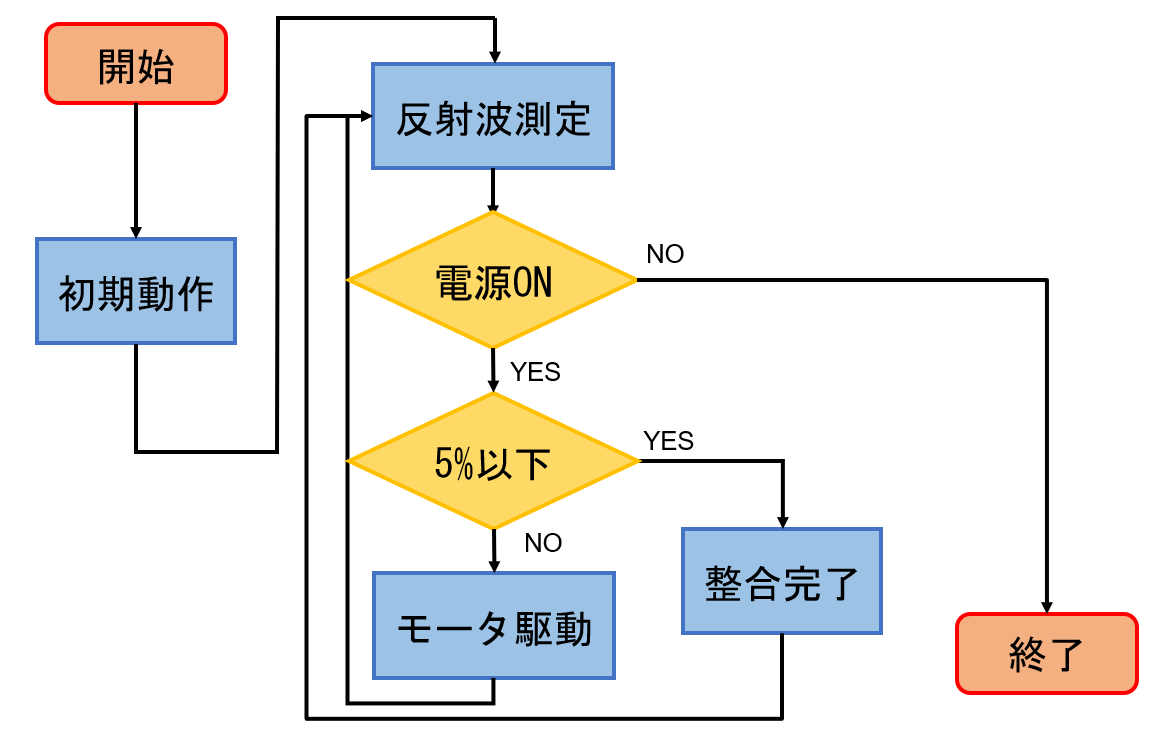
\includegraphics[width=18cm,height=15cm,clip,keepaspectratio]{3.10.png}
 \end{center}
 \caption{フローチャート}
 \label{fig:3.10}
\end{figure}

\newpage

 \subsection{Arduino周りの回路素子と配線}
 「Arduino R4」に接続される素子はモータを動かすための「モータドライバ」,初期位置を検出する「センサー」,
 「AC/DCコンバータ」,整合状況を表示する「LCD」,「LED」,また回路では方向性結合器がある.それらの配線を図3.8に示す.
 \begin{figure}[h!]
 \begin{center}
  \includegraphics[width=18cm,height=18cm,clip,keepaspectratio]{3.11.pdf}
 \end{center}
 \caption{Arduino周りの配線}
 \label{fig:3.11}
\end{figure}
%============================================================================================================
\chapter{自動整合器の動作と評価}
\section{使用機器}
以下に本研究で使用した機器を示す.\\\\
・ファンクションジェネレータ：SG-4105\\
・13.56MHz RF電源:23年度卒業研究製作\\
・直流可変電源 (0～160V):PAN160-3.5A\\
・オシロスコープ:DPO 2014B\\
・電力・SWR計:SX-100\\
・負荷抵抗（50Ω）:WELZ CT-300\\
\section{反射波検出部の評価}
\subsection{製作した方向性結合器}

\subsection{検波回路}
\section{自動整合器の評価}
%============================================================================================================
\chapter{総括}
\acknowledgment
本研究を遂行するにあたり,ご多忙の中,終始適切な助言を下さり,有意義な研究ができる環境を作ってくださった
喜屋武先生に感謝申し上げます.また,共同研究者である中尾君,貴船君の協力のおかげで私の至らない部分を
補いあいながら研究をやり遂げることができました.ありがとうございました.最後に,学生生活を支えてくれた両親
にもこの場を借りて感謝申し上げます.
\begin{thebibliography}{9}
       \bibitem{tandemmatch} John Grebenkemper,
       ``The tandem Match - An Accurate Directional Wattmeter,''
       QST, Vol.71, No.1, pp.18-26（1987）.

       \bibitem{w2aew_video} w2aew,
       ``\#196: How a Directional Coupler in an SWR meter works,''
       YouTube, \url{https://www.youtube.com/watch?v=byF1FLdbUiA} （2015）.

         \bibitem{ichikawa} 市川親司,
       ``複雑な実最適化問題への実践的アプローチ,''
       知的システムデザイン研究室, \url{http://mikilab.doshisha.ac.jp/dia/monthly/monthly04/20040628/ichikawa.pdf} （2004）.

       
       \bibitem{shuuri} 伊藤 康彦, 中野 治久, 星野 航希,
       ``高周波自動整合器の修理,''
       核融合科学研究者,名古屋大学大学院,（2024）.

       \bibitem{inaba} 稲葉 保,
       ``パワーMOSFETの高速スイッチング応用,''
       CQ出版社,（2011）.

       \bibitem{RF_power_source} 岩崎 智幸, 岩橋 拓美, 大河原 礼也, 
       ``ソフトスイッチングLC共振回路を用いた$150\, \mathrm{W}$級$13.56\, \mathrm{MHz}$高周波電源の製作,''
       近畿大学産業理工学部電気電子工学科,（2023）.

       \bibitem{match_coupler} エンジャー,
       ``方向性結合器の原理,''
       \url{https://engineer-climb.com/directional-coupler/}

       \bibitem{ozawa} 小澤 拓治,
       ``RF ワールド No.10 はじめてのネットワーク・アナライザ,''
       CQ出版社,（2010）.

       \bibitem{togawa_j} 戸川 治郎,
       ``スイッチング電源のコイル/トランス設計,''
       CQ出版社,（2012）.

       \bibitem{togawa_t} 外川 貴規,
       ``KiCADではじめる「プリント基板」製作,''
       工学社,（2018）.

       \bibitem{wakai} 若井 一顕,
       ``回路設計者のためのインピーダンス整合入門,''
       日刊工業新聞社,（2015）.

       \bibitem{photo_sensor} KI1233 データシート, 新光電子, 
       \url{https://akizukidenshi.com/goodsaffix/C_KI1233_KI1234_KI1235_KI1236_E.pdf}

       \bibitem{power_supply} RID-65 データシート, MEAN WELL, 
       \url{http://www.meanwelljapan.com/webapp/product/search.aspx?prod=RID-65}

       \bibitem{motor} ST-42BYH1004 データシート, Mercury Motor, 
       \url{https://akizukidenshi.com/goodsaffix/ST-42BYH1004-5013.pdf}

       \bibitem{moter_driver} TB67S249FTG データシート, 東芝デバイス\&ストレージ, 
       \url{https://www.pololu.com/product/3096}

\end{thebibliography}


\end{document}

%%% Local Variables:
%%% mode: yatex
%%% TeX-master: t
%%% End:
